\documentclass{beamer}
 
\usepackage[english]{babel}

\usepackage{graphicx}
\usepackage{wasysym}

\usepackage{amssymb}
\usepackage{bmpsize}




\newcommand{\Cells}{\mathcal{C}}
\newcommand{\Edges}{\mathcal{E}}
\newcommand{\Facets}{\mathcal{F}}
\newcommand{\Points}{\mathcal{P}}
\newcommand{\Vertices}{\mathcal{V}}
 


\title[]{Example of Beamer to Powerpoint conversion  }
\author{ Anonymous author}
\institute{No institution }


\begin{document}




\begin{frame}[plain]
\titlepage
\end{frame}

\begin{frame}
\frametitle {First Slide}
this is an itemize example: 
\begin{itemize}
\item first item
\item second item
\item third item
\end{itemize} 
\end{frame}



\begin{frame}
\frametitle {Slide with images}
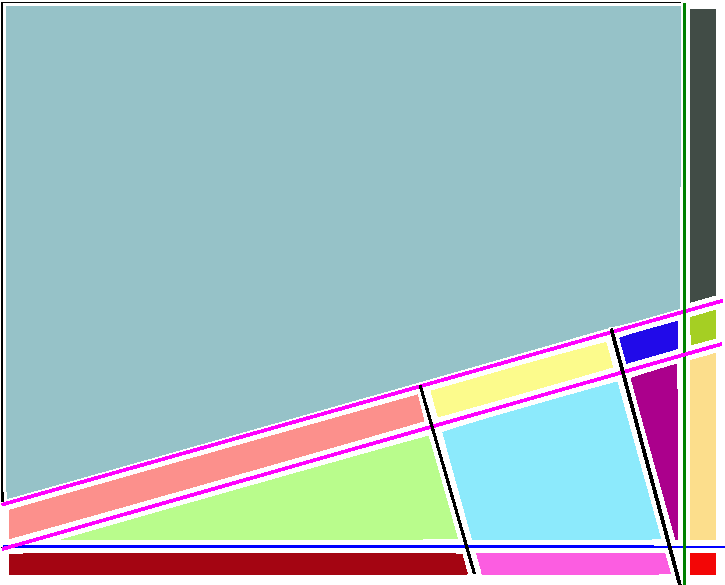
\includegraphics[width=0.45\linewidth]{image.pdf}
\end{frame}

\begin{frame}
\frametitle {Equations}
$$f(a,b)=\sum_i (ax_i-b)^2$$
\end{frame}
  
\end{document}



